
\section{Theorie}
\label{sec:Theorie}

%Abb.1
 Es  Zum anderen kann die LC-Kette auch als System gekoppelter
    Schwingungssysteme betrachtet werden, welches viele Eigenschwingungen besitzt.
     Desweiteren können Wellenpakete auf ihr übertragen werden.
     Da ein Wellenpaket aus einer Menge unterschiedlicher Einzelwellen besteht
      und jede von diesen eine eigene Phasengeschwindigkeit besitzt, kommt es zu einer Verzerrung
  der gestalt des Wellenpaketes. Diesen Effekt nennt man Dispersion.


     \begin{figure}[H]
       \centering
       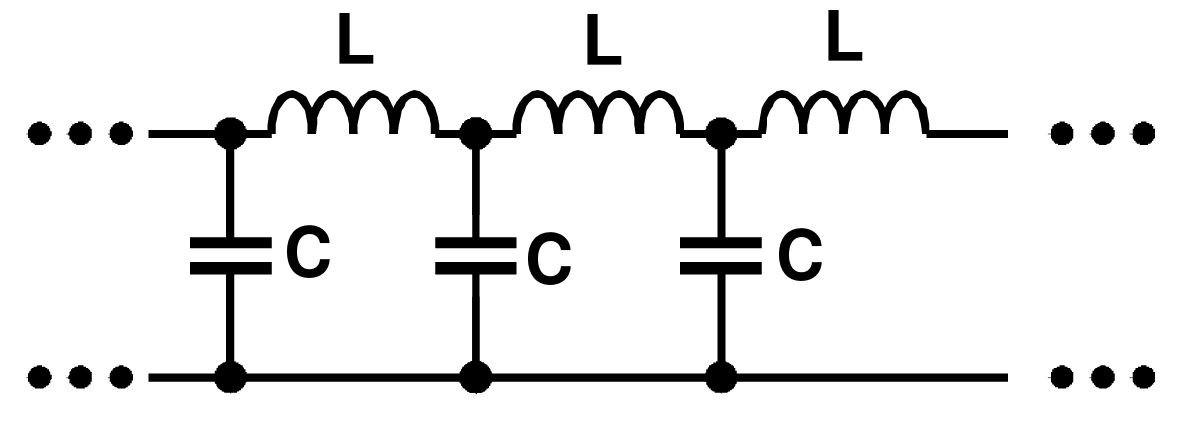
\includegraphics[width=\linewidth-300pt,height=\textheight-300pt,keepaspectratio]{content/Grafiken/LCKette.png}
       \caption{Die unendliche LC-Kette}
       \label{fig:LC-Kette}
     \end{figure}

\subsection{Die stationäre LC-Kette}
Eine LC-Kette beschreibt eine Verkettung von n in Reihe geschalteten LC-Gliedern.
 Jeder dieser Glieder hat die Eigenschaften eines Tiefpasses, welcher
  Wechselspannungen mit geringen Frequenzen passieren lässt, hochfrequente jedoch
   verschwinden. Eine unendliche LC-Kette kann zudem als Ersatzschaltplan einer
    verlustfreien elektrischen Leitung angesehen werden. Eine weitere Eigenschaft
     liegt in der Existenz des Wellenwiderstandes:
     \begin{equation}
       Z(f) = \sqrt{\frac{L}{C}} \cdot \frac{1}{2\pi \sqrt{1-0,25\omega² LC}}
     \end{equation}

1. Fall :Die einfache $LC$-Kette


Aus den kirchhoffschen Regeln folgt die BewegungsDGL:
\begin{equation}
- \omega ^2 C U_n + \frac{1}{L} \left( -U_{n-1} + 2U_ n -U{n-1} \right) = 0
\end{equation}

Mit einem komplexen E-Ansatz erhält man:
\begin{equation}
\omega ^2 = \frac{1}{2LC\pi^2}(1-cos\theta)
\end{equation}
Dieser Ausruck wird als Dispersionsrelation beschrieben und stellt die Änderung
 der Phase pro Kettenglied in Abhängigkeit der Frequenz dar. Anhand der Formel lässt sich erkennen,
  dass der Frequenzbereich indem Schwingungen auftreten begrenzt ist. Für Frequenzen >
 $\frac{1}{\sqrt{2LC\pi^2}}$ bilden sich daher keine Schwingungen aus.\\\\

 2. Fall: Die $LC_1C_2$-Kette:
 Aus den kirchhoffschen Regeln folgen die BewegungsDGLn:
 \begin{equation}
   -\omega^2 C_1 U_{2n+1} + \frac{1}{L} \left( -U_{2n} + 2U_{2n+1} - U_{2n+2} \right) = 0
 \end{equation}
 und
 \begin{equation}
   -\omega^2 C_2 U_{2n} + \frac{1}{L} \left( -U_{2n-1} + 2U_{2n+1} - U_{2n+1} \right) = 0
 \end{equation}

Es folgt für die auftretende Dispersion:
\begin{equation}
  f_{1/2}^2 = \frac{1}{4\pi^2L}\left(\frac{1}{C_1}+\frac{1}{C_2}\right) \pm \frac{1}{4\pi^2L}\sqrt{\left(\frac{1}{C_1}+\frac{1}{C_2} \right)^2 - \frac{4 sin^2\theta}{C_1C_2}}
\end{equation}
Es zeigt sich, dass die $C_1C_2$-Kette aufgrund der positiven und negativen Versionen der Wurzel
zwei Frequenzbereiche besitzt in denen Schwingungen auftreten. Die Verläufe der Unteren und Oberen
 Grenzfrequenz werden akustischer bzw. optischer Ast genannt. Nähert man den Verlauf mit $sin \theta \approx \theta$ erhält man eine Kurvenverlauf, welcher dann ca so aussieht.

 \begin{figure}[H]
   \centering
   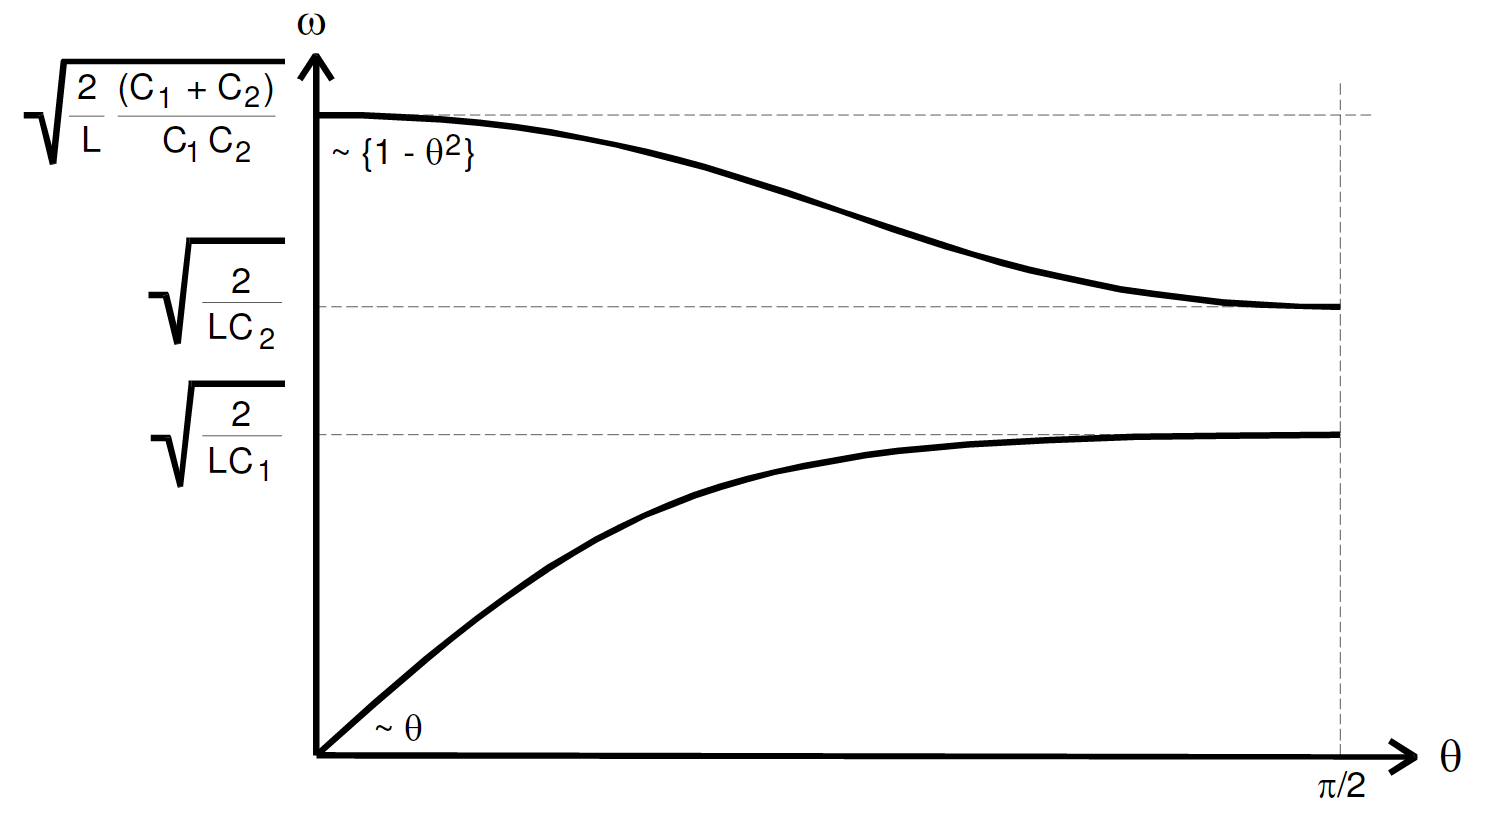
\includegraphics[width=\linewidth-200pt,height=\textheight-200pt,keepaspectratio]{content/Grafiken/Dispersionskurven.png}
   \caption{Die nötige Frequenz in Abhängigkeit der Dispersion}
   \label{fig:LC-Kette}
 \end{figure}


\subsection{Die Eigenschaften einer endlichen LC-Kette}
Liegt eine LC-Kette endlicher Länge vor, bzw wurden Anfangs und Endwiderstand
 nicht nach Formel () der Frequenz des Wechselsstromes ensprechend angepasst,
  kommt es zur Reflexion ankommender Wellen. Aus den kirchhoffschen Regeln folgt das Verhältnis:
  \begin{equation}
    \frac{U_ref}{Uein} = \frac{R-Z}{R+Z}\text{.}
  \end{equation}
  Es folgen die Spezialfälle:\\
  a) Die LC-Kette besitzt ein offens Ende, $R$ beträgt also $\infty$. An diesem
   wird eine ankommende Welle vollständig und ohne Phasensprung reflektiert.\\

  b) Die LC-Kette ist kurzgeschlossen, $R$ beträgt daher 0. An diesem Ende wird
   eine ankommende Welle vollständig, jedoch mit einem Phasensprung von $\pi$ reflektiert.\\

 c) Werden Anfangs und Endwiderstand auf den Wellenwiderstand der LC-Kette eingestellt, verhält
  sich die endliche wie eine unendliche LC-Kette. Aus diesem Grund kommt es auch nicht zur Reflexion.
